%!TEX root = main.tex

\section{Neutron Binding Energy} % (fold)
\label{sec:neutron_binding_energy}

\subsection{Sodium Iodide Detector} % (fold)
\label{ssub:sodium_iodide_detector}
The sodium iodide detector is a scintillation detector that uses a NaI crystal doped with thallium to create scintillation photons when a gamma ray photon hits the crystal. The thallium is added as an activator to provide extra available energy levels for the photons in the crystal to occupy. In the pure state, the NaI has a large forbidden band gap between the conduction and valence bands, shown in figure \ref{fig:thaliumactivator}. The activator reduces this gap so that an emitted photon is in the range that the photomultiplier tube is sensitive to, typically visible.
\begin{figure}[ht]
	\centering
	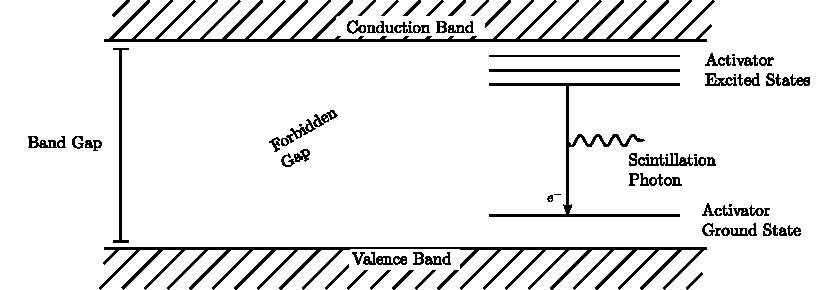
\includegraphics[width=0.9\textwidth]{NaIbands.pdf}
	\caption{The element thallium is added to the pure crystal of sodium iodide to provide extra energy levels for the electrons, which sit inside the forbidden gap of the crystal latice structure. These allow a photon of a useful wavelength to be emitted when electron decays to a lower energy.\label{fig:thaliumactivator}}
\end{figure}

When a gamma photon enters the detector it ionises a molecule of NaI creating excited states in the crystal that then decay via visible photons. The number of photons that are produced is proportional to the energy of the incident photon, as the energy of the gamma ray increases, more scintillation photons are produced. Thus, the energy of the original can be found be counting the number of photons produced. 

These scintillation photons are used to create electrons which are more easily counted. At the photo-cathode, the photons release electrons via the photoelectric effect. The electrons are then passed through the photomultiplier tube which increases the number of photons linearly by accelerating them through a high potential difference so they can knock more electrons out from the dynodes (see figure \ref{fig:naidetctor}). This results in a stream of electrons that can be measured, and which is proportional to the original energy of the photon via the number of scintillation photons, the number of electrons and the multiplication factor of the increase of electrons from the PM tube. Since each of these steps is a linear relationship, a calibration setting can be taken using known results, and a simple linear equation relating the reading taken to the energy of the photon found.
\begin{figure}[ht]
	\centering
	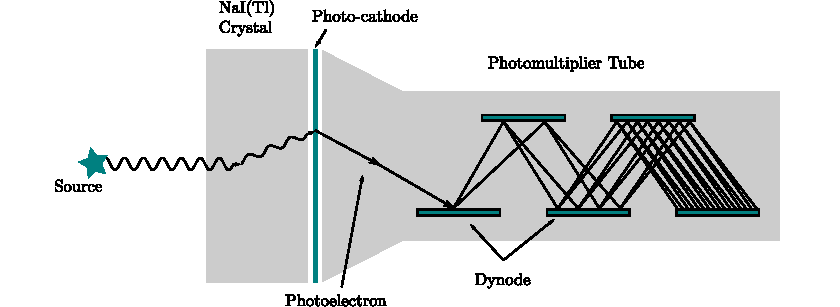
\includegraphics[width=0.9\textwidth]{NaIdetector.pdf}
	\caption{The sodium iodide detector is a commonly used gamma ray detector that uses the relationship between the energy of a photon and the ionisation power that it has to measure its energy via a calibration equation.\label{fig:naidetctor}}
\end{figure}

The detector requires a high voltage which is placed across the dynodes and the anode to accelerate the electrons once they have entered the PM tube. Using this method of acceleration and re-acceleration, the photomultiplier tube is able to increase the number of electrons by a factor of roughly $10^5$ depending on the voltage bias.
\begin{figure}[ht]
	\centering
	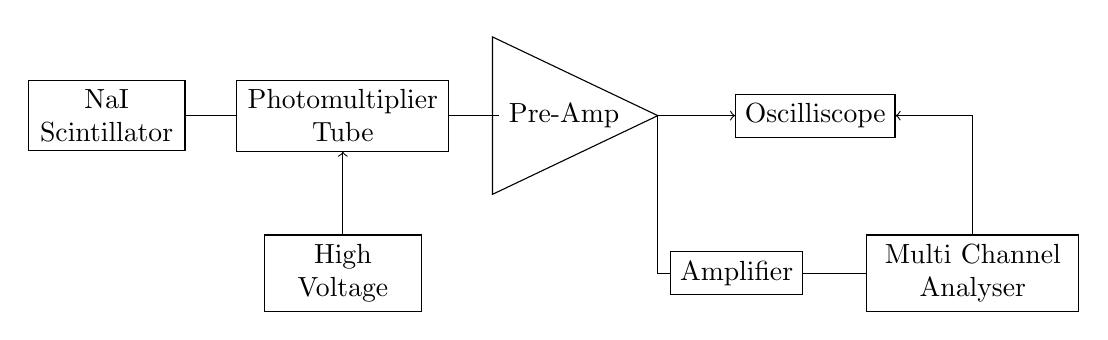
\begin{tikzpicture}
    \node[rectangle, draw, text centered, text width=5em] (1) at (2,0) {NaI Scintillator};
	\node[rectangle, draw, text centered, text width=7em] (2) at (5,0) {Photomultiplier Tube};
	\node[rectangle, draw, text centered, text width=5em] (3) at (5,-2) {High Voltage};
	\node (4) at (7.81,0) {Pre-Amp};
	\node (tri1) at (6.9,1) {	};
	\node (tri2) at (9,0) {	};
	\node (tri3) at (6.9,-1) {};
	\draw (tri1.center) -- (tri2.center) -- (tri3.center) -- cycle;  
	\node[rectangle, draw] (5) at (11,0) {Oscilliscope};
	\node[rectangle, draw] (6) at (10,-2) {Amplifier};
	\node[rectangle, draw, text centered, text width=7em] (7) at (13,-2) {Multi Channel Analyser};
	\draw (1) -- (2);
	\draw[<-] (2) -- (3);
	\draw (2) -- (4);
	\draw[->] (tri2.center) -- (5);
	\draw (6) -| (tri2.center);
	\draw (6) -- (7);
	\draw[->] (7) |- (5);
\end{tikzpicture}
\end{figure}

% subsubsection sodium_iodide_detector (end)

\subsection{Calibration} % (fold)
\label{sub:calibration}
Before any data can be read from the spectra taken from the detector, the data has to be calibrated. To do this, a set of known samples with well defined peaks is used to get a relation between the channel number of an observed peak and its energy. Once this is done, a relation can be found that relates the channel number to energy for use on later measurements.

The elements that were used included cobalt, barium, caesium, europium and americium. Each of these elements were available to measure, and each has recorded and accepted peaks that are at well defined positions. The data was taken from the National Nuclear Data Centre (NNDC). The table below, table \ref{tab:calibdata}, shows the data that we collected from these sources. The channel number refers to the position in the spectrum that the peak was observed and the expected peak is the energy of the peak that the respective peak is estimated to correspond to.

\begin{table}[ht]
	\centering
	\begin{tabular}{r c|c|c}
		\multicolumn{2}{c|}{Element} & Channel Number & Expected Peak Energy (keV) \\
		\hline\hline
		Cobolt 		& $\ce{^{60}Co}$  & 369.4	& 1332.0 \\
					&				  & 324.9	& 1173.0	\\
		\hline
		Barium		& $\ce{^{133}Ba}$ & 102.9	& 356.0	\\
					&				  & 86.08	& 302.9		\\
		\hline
		Caesium		& $\ce{^{137}Cs}$ & 188.4	& 661.7 \\
		\hline
		Europium	& $\ce{^{152}Eu}$ & 99.84	& 344.3 \\
					&				  & 222.0	& 778.9		\\
					&				  & 274.9	& 964.1		\\
					&				  & 311.0	& 1121/1086	\\
					&				  & 394.1	& 1408.0	
	\end{tabular}
	\caption{Several elements were used to measure a calibration relation that links the observed channel number to the energy.\label{tab:calibdata}}
\end{table}
From these, the graph in figure \ref{fig:naicalib} can be drawn which shows the relation that can be used as a calibration between energy and channel number. The exact value of this relation, intercept and gradient, are subject to change since the calibration is retaken at the start of each session to account for changes in the experimental set-up and the radioactivity of the source which will decrease with time.

\begin{figure}[ht]
	\centering
	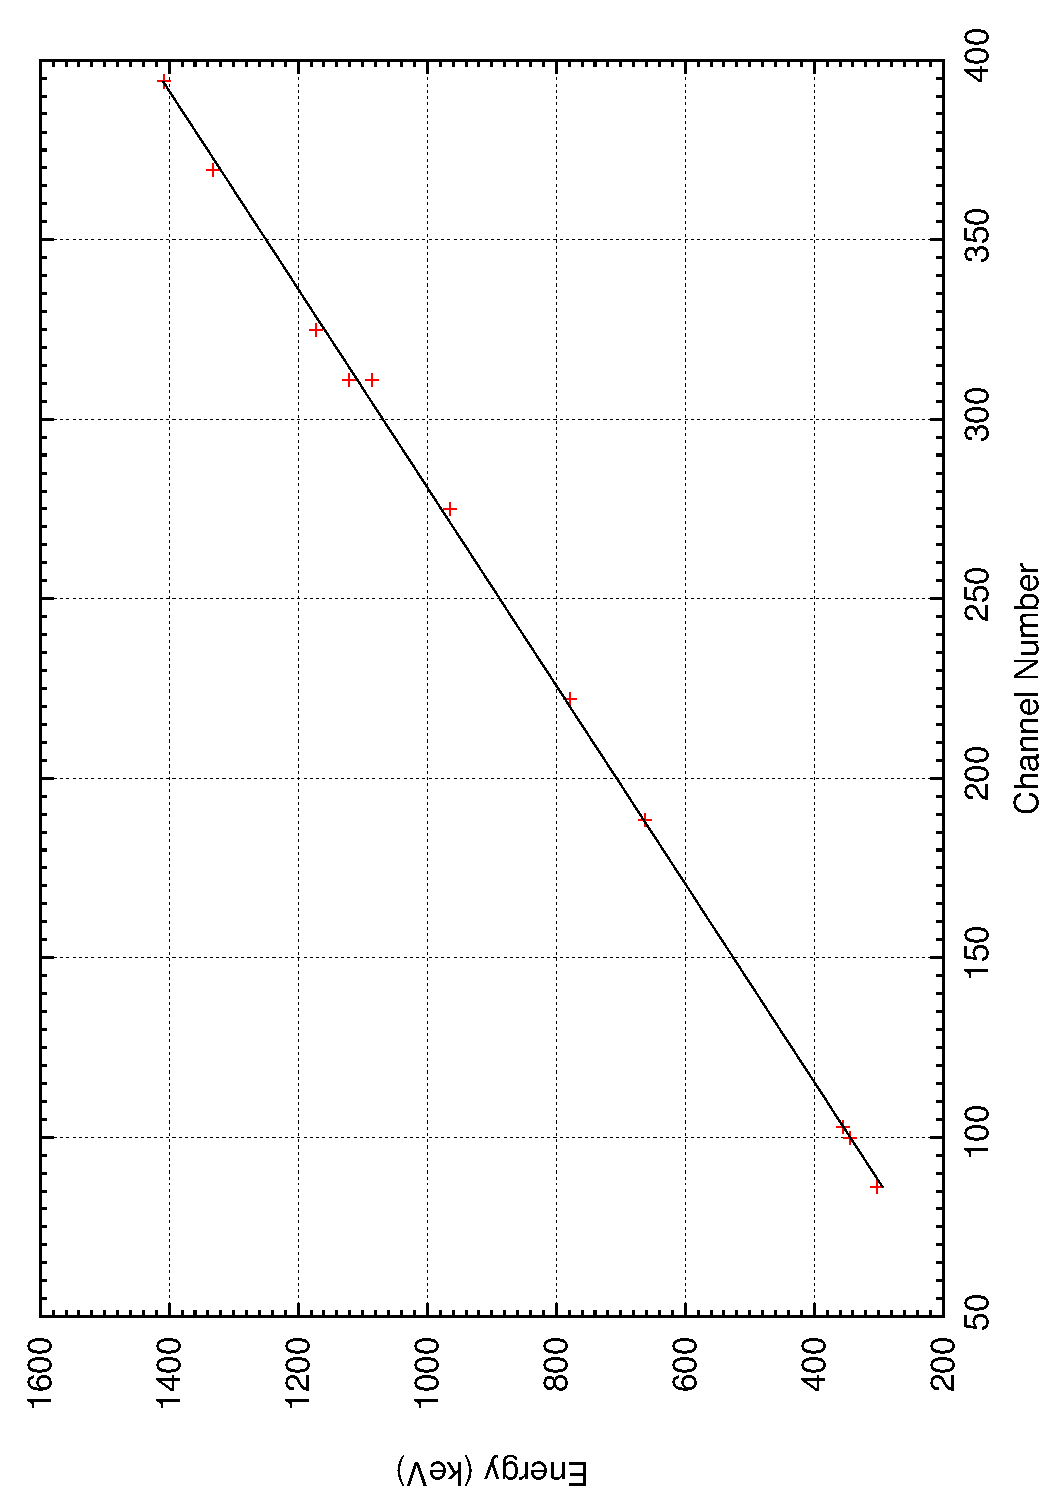
\includegraphics[angle=270,width=0.6\textwidth]{calibration1NaI.pdf}
	\caption{The sodium iodide detector provides a channel number readout that is directly proportional to the energy of the corresponding reaction event. Thus, using known data points, a relation between channel number and energy can be found.\label{fig:naicalib}}
\end{figure}
An example of the spectra from the sources is shown in figure \ref{fig:cobaltcalib}. This shows the spectrum of $\ce{^{60}Co}$ which has been fitted with the Gaussian peaks to find the position and FWHM using the ``root'' package.

\begin{figure}[ht]
	\centering
	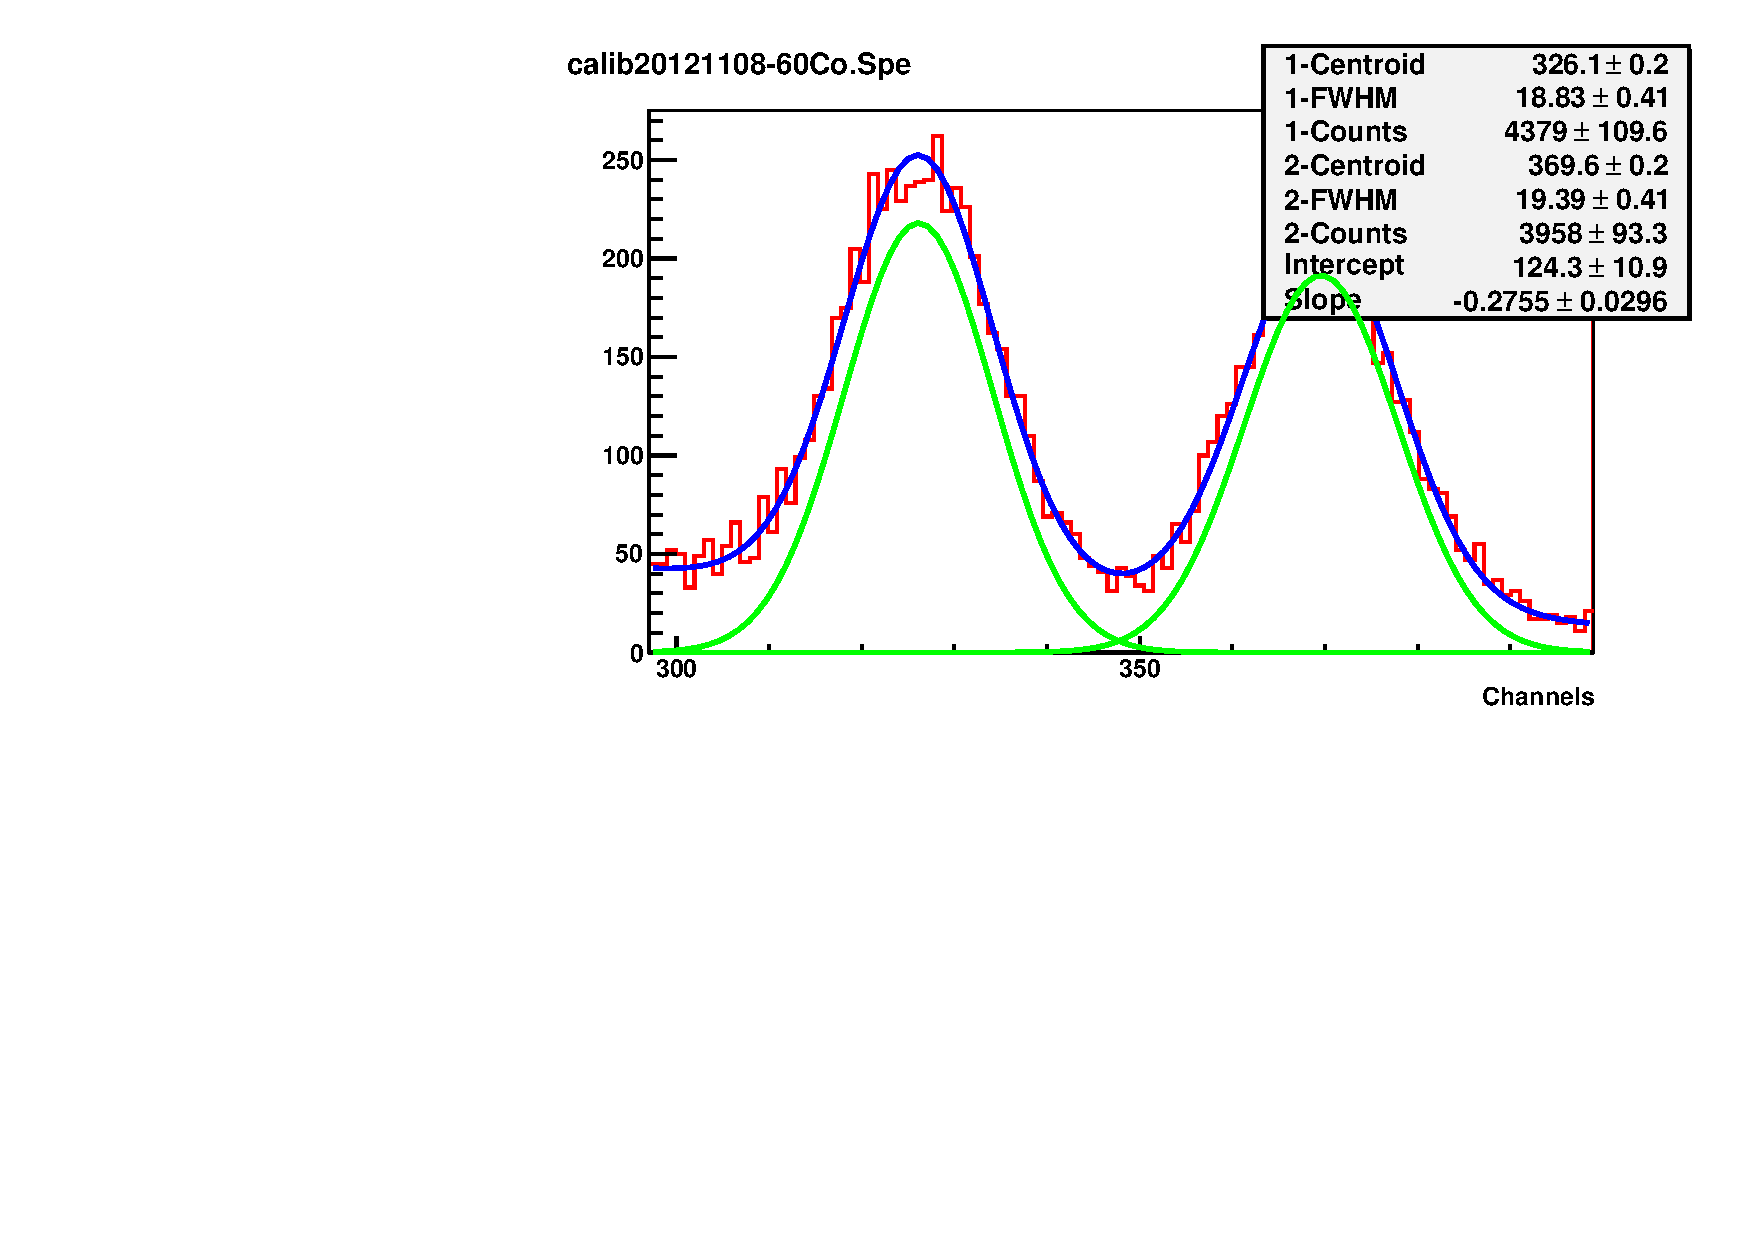
\includegraphics[width=0.7\textwidth]{calib20121113-60Co.pdf}
	\caption{An example of the peak for the radioactive element cobalt-60. These two peaks are well defined and have well known values. This means that they are good for using as calibration points for the detector.\label{fig:cobaltcalib}}
\end{figure}

This line has the equation,
\begin{align}
	E &= 3.63\times x - 18.31 \label{eq:calibNaI}
\end{align}
This equation, equation \ref{eq:calibNaI}, shall be used as the calibration equation for the sodium iodide experiment. The calibration was re-taken at the start of each session using the NaI detector, so this value represents the session where the actual experimental results were taken for the main section of finding the deuteron binding energy.
% subsection calibration (end)

\subsection{Energy Resolution} % (fold)
\label{sub:energy_resolution}
Scintillation detectors, such as the NaI detector in use here, have a relatively poor energy resolution. Statistical broadening of the peaks is usually the dominant form of broadening. When a reaction takes place, and so energy is deposited, in the scintillator crystal, the efficiency can be as low as around 10\%. This means that a far smaller amount of energy is actually transferred to the crystal than the energy of the incoming particle.

When the reaction takes place in the crystal, a number of photons, proportional to the energy deposited, are produced. But some of them are lost before they can reach the photomultiplier tube further reducing the measured number of photons. This also means that there is a minimum in the number of photons just before the photomultiplier tube. Since the number of arriving photons will be subject to statistical fluctuations, the standard deviation in the photons reaching the PM tube is given by equation \ref{eq:standarddevgamma},
\begin{align}
	\text{Standard Deviation, }\sigma &= \sqrt{\text{Number of photons reaching the PM tube}}\label{eq:standarddevgamma}
\end{align}
Since this is proportional to the energy of the original photon that caused the reaction, it can be shown that
\begin{align}
	R &= \frac{\text{FWHM}}{H_0} \\
	&= k\frac{\sqrt E}{E} = \frac{k}{\sqrt E}
\end{align}
Where FWHM is the full width at half maximum of any given peak, $H_0$ is the height of the peak and $k$ is a constant of proportionality. This means that the resolution can be easily observed by plotting a graph of $\log k$ against $\log E$, which should give a slope of $-\frac{1}{2}$ in an ideal case.

The resolution of the NaI detector is use was measured using the method described above.
% subsection energy_resolution (end)

\subsection{Neutron Binding Energy} % (fold)
\label{sub:neutron_binding_energy}
The first full experiment that was attempted was measuring the binding energy of neutrons by observing the $\gamma$-ray emitted when the neutrons are captured by protons in the water surrounding a neutron source via reaction \ref{eq:neutronbinding},
\begin{align}
	\cf{^{1}_{1}p} + \cf{^{0}_{1}n} &\rightarrow \cf{^{1}_{2}d} + \gamma \label{eq:neutronbinding}
\end{align}

The exact energy would be found from the peak from this photon observed in the spectrum.

In order to observe the spectrum as clearly as possible, the experiment was run overnight collecting data for approximately 25 hours. This would give us a much clear spectrum and so lower errors on the final data. The spectrum that was recorded is shown in figure \ref{fig:tank-full_spectrum}, along with a description of each of the major peaks that are visible. This plot is shown on a single $\log y$ axis so that the peaks are more easily discernible.
% \begin{figure}[ht]
% 	\centering
% 	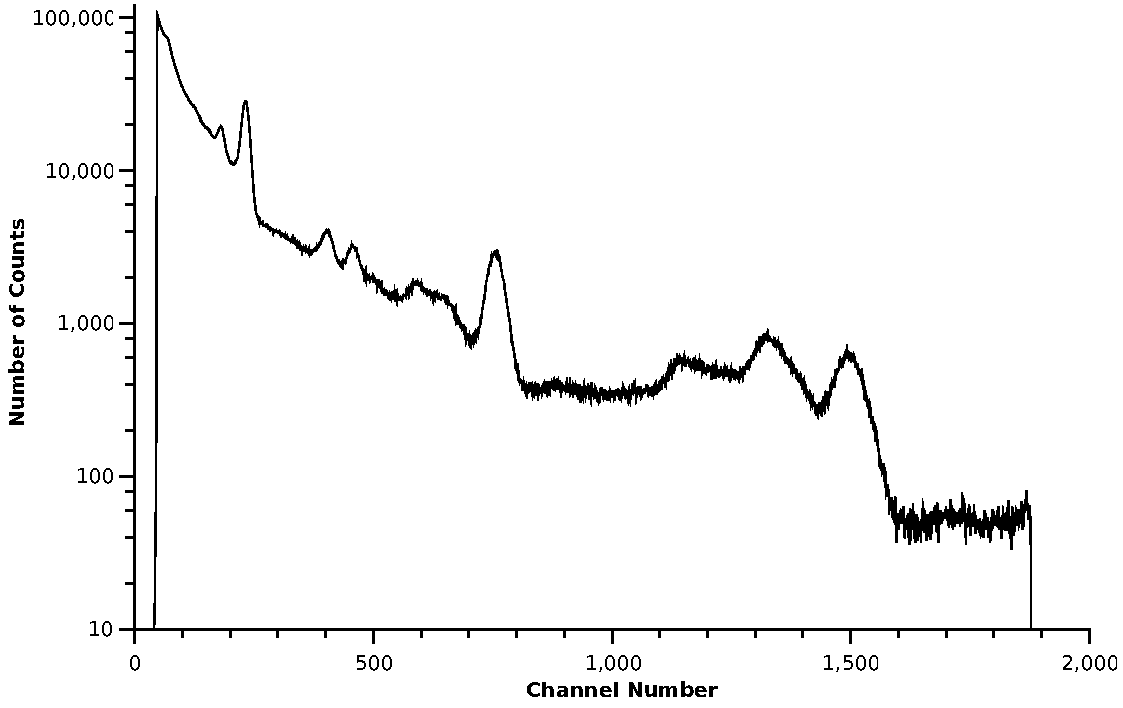
\includegraphics[width=0.9\textwidth]{tank-full_spectrum.pdf}
% 	\caption{The spectrum from the neutron tank observing a radioactive neutron emitter for a prolonged period.
% 	\label{fig:tank-full_spectrum}}
% \end{figure}
% \begin{figure}[ht]
%   \centering
%   \begin{overpic}[width=0.9\textwidth]{tank-full_spectrum.pdf}
%     \put(22,54){1}
%     \put(19,52.5){2}
%     \put(28,43){3}
%     \put(32,42){4}
%     \put(45,41){5}
%     \put(40,38){6}
%     \put(36,39){7}
%     \put(76,33){8}
%     \put(68,35){9}
%     \put(61,32){10}
%   \end{overpic}
%   \caption{The spectrum from the neutron tank observing a radioactive neutron emitter for a prolonged period of time.
%   \label{fig:tank-full_spectrum}}
% \end{figure}

\begin{figure}[ht]
  \centering
  \begin{overpic}[width=0.9\textwidth]{tank-full_spectrum_overnight.pdf}
    \put(20,57){1}
    % \put(19,52.5){2}
    \put(32,46){2}
    \put(36,44){3}
    \put(49,49){4}
    \put(44,43){5}
    \put(40,45){6}
    \put(85,36){7}
    \put(76,38){8}
    \put(66,36){9}
  \end{overpic}
  \caption{The spectrum from the neutron tank observing a radioactive neutron emitter for a prolonged period of time.
  \label{fig:tank-full_spectrum}}
\end{figure}

The major peaks, from figure \ref{fig:tank-full_spectrum} are as follows:
	\begin{enumerate}\itemsep1pt \parskip0pt \parsep0pt
		\item 511\,keV peak from the electron rest mass.
		% \item Unknown.
		\item Unknown.
		\item Double escape peak?.
		\item \textbf{Neutron binding energy}.
		\item Unknown
		\item Single escape peak from the neutron binding energy.\\
		Double escape peak from the neutron binding energy.
		\item Reaction peak from either oxygen ($\ce{^8O_2}$) or carbon ($\ce{^{12}C}$) from the water in the tank. Further investigation would be needed to determine the exact cause of this peak since it is so weak in comparison to the others.
		\item Escape peak from the carbon/oxygen peak
		\item Double escape peak from the carbon/oxygen peak
	\end{enumerate}

\subsubsection{Escape Peaks} % (fold)
\label{ssub:escape_peaks}
The peaks that are labelled as ``escape peaks'' from the previous graph, figure \ref{fig:tank-full_spectrum}, are due to the phenomena called pair production. Pair production occurs if the incident energy is above 1022\,keV, i.e.\ twice the rest mass of the electron, and results in the production of two 511\,keV annihilation gamma rays. If one of these gamma rays escapes the detector while the other is completely absorbed, 511\,keV will be lost from the detector. This results in a separate peak in the spectrum representing the original energy minus 511\,keV. This is called a single escape peak. If both annihilation gamma-rays escape the detector a double escape peak is formed with an energy of the expected energy minus $2\times$ 511\,keV, or 1022\,keV.

Escape peaks can seen whenever there are events with energies greater than the 1022\,keV limit. They are generally slightly lower in height than the main peak and are always at the same distance from the main peak.
% subsubsection escape_peaks (end)

\subsubsection{Background Radiation} % (fold)
\label{ssub:background_radiation}
This experiment was carried out using a sample of americium-beryllium (AmBe) and as such, the peaks seen in the resulting spectrum should be well known and well defined. Instead, there are a number of peaks that cannot, at the present time, be accounted for. There are several explanations to explain these peaks. 
\begin{enumerate}
	\item The first is the method of creating the samples in use. The samples were made by bombarding the metals using a synchrotron particle accelerator. This has the effect of possibly creating an impure sample so that there are other elements that are decaying producing their own spectrum that is adding the the expected one.
	\item Another possibility is that the other radiation sources that are stored nearby introduced extra peaks from their own radioactive decays.
\end{enumerate}
% subsubsection background_radiation (end)

\subsection{Experimental Results} % (fold)
\label{sub:experimental_results}
The calibration data that was taken gave a channel number-energy relation of
\begin{align}
	E &= 3.63\times C - 18.31
\end{align}
where $E$ is the actual energy and $C$ is the observed channel number. Using this equation, peak number 5 from the above spectrum, figure \ref{fig:tank-full_spectrum}, is found to lie at an energy of $2.244\pm0.048$\,MeV. The data taken from the spectrum is shown in table \ref{tab:tankdata}. This table shows the channel number of each of the peaks labelled above, the error on this position, the energy and corresponding error for the peak and the differences between some of the adjacent peaks. This last column is used to verify escape peaks which are always at 511\,keV below the main peak.
\begin{table}[ht]
	\centering
	\begin{tabular}{c|c|c|c|c}
		Channel \textnumero & Error on Channel \textnumero & Energy & Error on Energy & Difference \\
		\hline\hline
		181.20 & 0.07 & 496 & 31 & \\
		232.45 & 0.02 & 651 & 32 &  \\
		403.33 & 0.15 & 1170 & 36 &  \\
		458.6 & 0.18 & 1338 & 38 &  \\
		617.3 & 0.56 & 1820 & 43 & 482 \\
		757.2 & 0.08 & 2244 & 48 & 425 \\
		1168.5 & 13.0 & 3492 & 66 & 1248 \\
		1335.4 & 0.50 & 3999 & 73 & 507 \\
		1496.6 & 0.28 & 4488 & 81 & 489
	\end{tabular}
	\caption{Values for the channel numbers and corresponding energies of the peaks from the spectrum of the BeAm sample in the water tank.\label{tab:tankdata}}
\end{table}

The values for the channel numbers, along with the corresponding errors, in table \ref{tab:tankdata}, were taken from the results of the peak fitting algorithm, ``Buffit'', provided as an extension to be used with the ``root'' interpreter framework. An example of this peak fitting is shown below in figure \ref{fig:tankspecbuffit}.

The value for the errors on the energies calculated here are given equation \ref{eq:caliberrors}.
\begin{align}
	\left(\sigma E\right)^2 &= \left(\sigma Ch\times m\right)^2 + \left(\sigma m\times Ch\right)^2 + \left(\sigma c\right)^2 \label{eq:caliberrors}	
\end{align}
where
\begin{description}
	\item[$\sigma E$] is the error on the energy
	\item[$Ch$] is the channel number from the detector
	\item[$m$] is the gradient of the line fit of the data
	\item[$c$] is the intercept of the line fit.
\end{description}

\begin{figure}[ht]
	\centering
	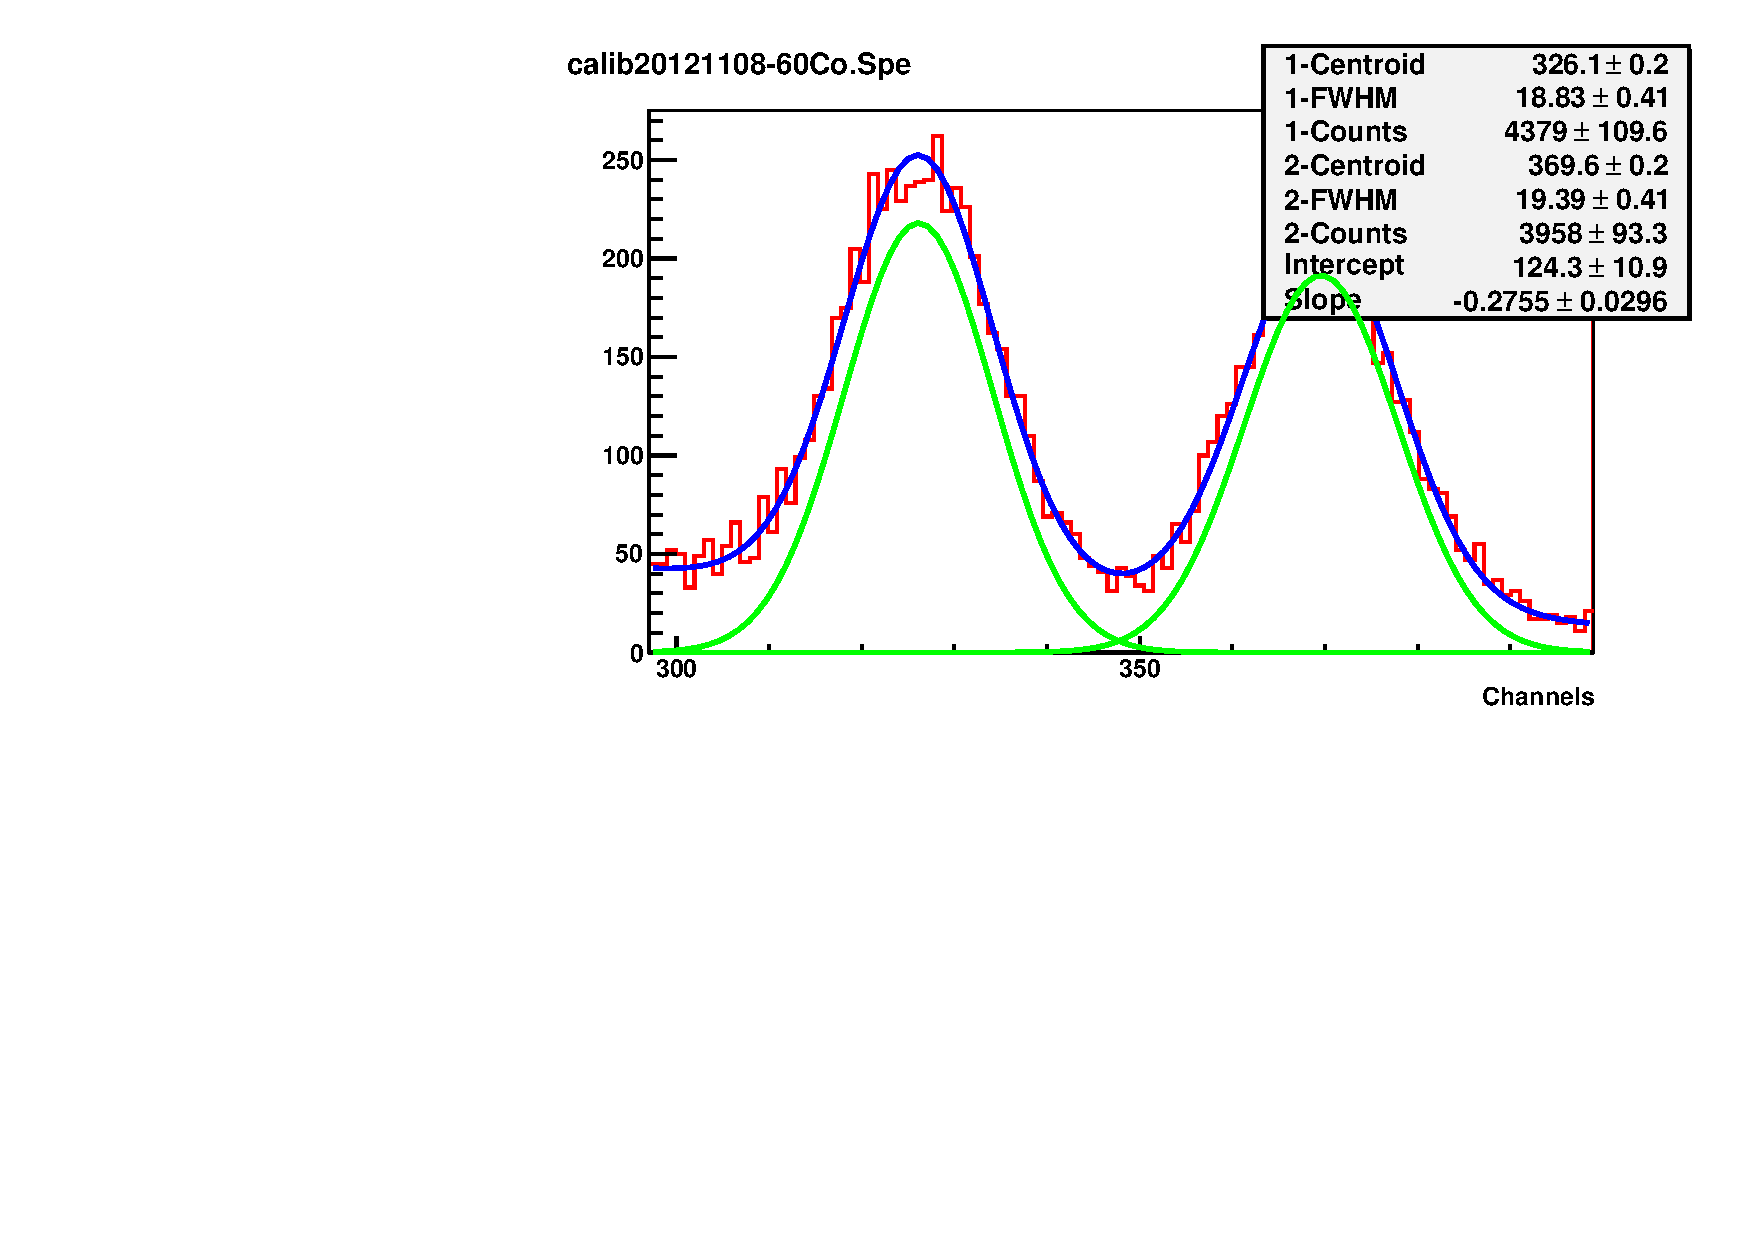
\includegraphics[width=0.7\textwidth]{calib20121113-60Co.pdf}
	\caption{An example of the peak for the radioactive element cobalt-60. These two peaks are well defined and have well known values. This means that they are good for using as calibration points for the detector.\label{fig:tankspecbuffit}}
\end{figure}

% subsection experimental_results (end)

\subsection{Analysis of Experimental Results} % (fold)
\label{sub:analysis_of_experimental_results}
The binding energy of the deuteron can be found theoretically from the mass difference between the deuteron and its individual components, as follows.
\begin{align}
	\ce{^1_0 n} + \ce{^1_1 p} &\rightarrow \ce{^2_1 d} + \gamma
\end{align}
The mass excess of each of these is as follows
\begin{align*}
	\Delta \ce{^1 p} &= 7.2889 \text{MeV} \\
	\Delta \ce{^1 n} &= 8.0713 \text{MeV} \\
	\Delta \ce{^2 d} &= 13.1357 \text{MeV}
\end{align*}
The binding energy is thus
\begin{align}
	7.2889 + 8.0713 + 13.1357 &= 2.2245 \text{MeV}
\end{align}
We can also find the difference between the binding energy of $\ce{^{16}O}$ and $\ce{^{17}O}$ from
\begin{align}
	\ce{^{16}_8 O} + \ce{^1_0 n} \rightarrow \ce{^{17}_8 O} + \gamma
\end{align}
For this reaction, the mass excesses are
\begin{align*}
	\Delta \ce{^{16} O} &= -4.7370 \text{MeV} \\
	\Delta \ce{^{17} O} &= -0.8087 \text{MeV} \\
	\Delta \ce{^1 n} &= 8.0713 \text{MeV} \\
\end{align*}

This confirms that the peak labelled number 4 is indeed in the correct energy location to be the binding energy of the neutron, and provides good evidence that the final unknown peak, peak number 7, could be from the oxygen in the water in the tank.
% subsection analysis_of_experimental_results (end)
% subsection neutron_binding_energy (end)

% section neutron_binding_energy (end)

